% =========================================================
\section{Experimental Design}
\label{sec:experiments}
% =========================================================
% 重点检查一下benchmark前面的形容词，感觉好几个地方不一样
\subsection{Temporal O\&M Benchmark}
\label{sec:dataset}

% BEFORE: We construct a semantic benchmark for controlled evaluation of temporal evidence retrieval in dynamic O\&M scenarios.
We construct a public-source-grounded synthetic temporal O\&M benchmark for controlled evaluation of temporal evidence retrieval in dynamic O\&M scenarios. The dataset is constrained by public-source background information and constructed with artificial intelligence (AI) assistance; it is not derived from real power-station fault logs and is not a real O\&M dataset manually annotated by domain experts. \revhl{We use public product documents and research datasets to constrain cell type, typical physical ranges, and sampling background. The O\&M events, diagnostic changes, procedure contexts, and queries are then synthesized under these constraints. We include late-arriving records, supersession, cross-source complementary evidence, multi-episode ambiguity, and persistent uncertainty as controlled conditions for comparing retrieval methods.}

\revhl{Figure~\ref{fig:benchmark_design} traces the construction from public-source constraints to synthetic O\&M event chains. Each chain supplies the records to be retrieved and the events about which queries are asked. We annotate each query with a reference evidence flow and a structured reference answer, used for retrieval and generation evaluation, respectively.}

\begin{figure*}[t]
    \centering
    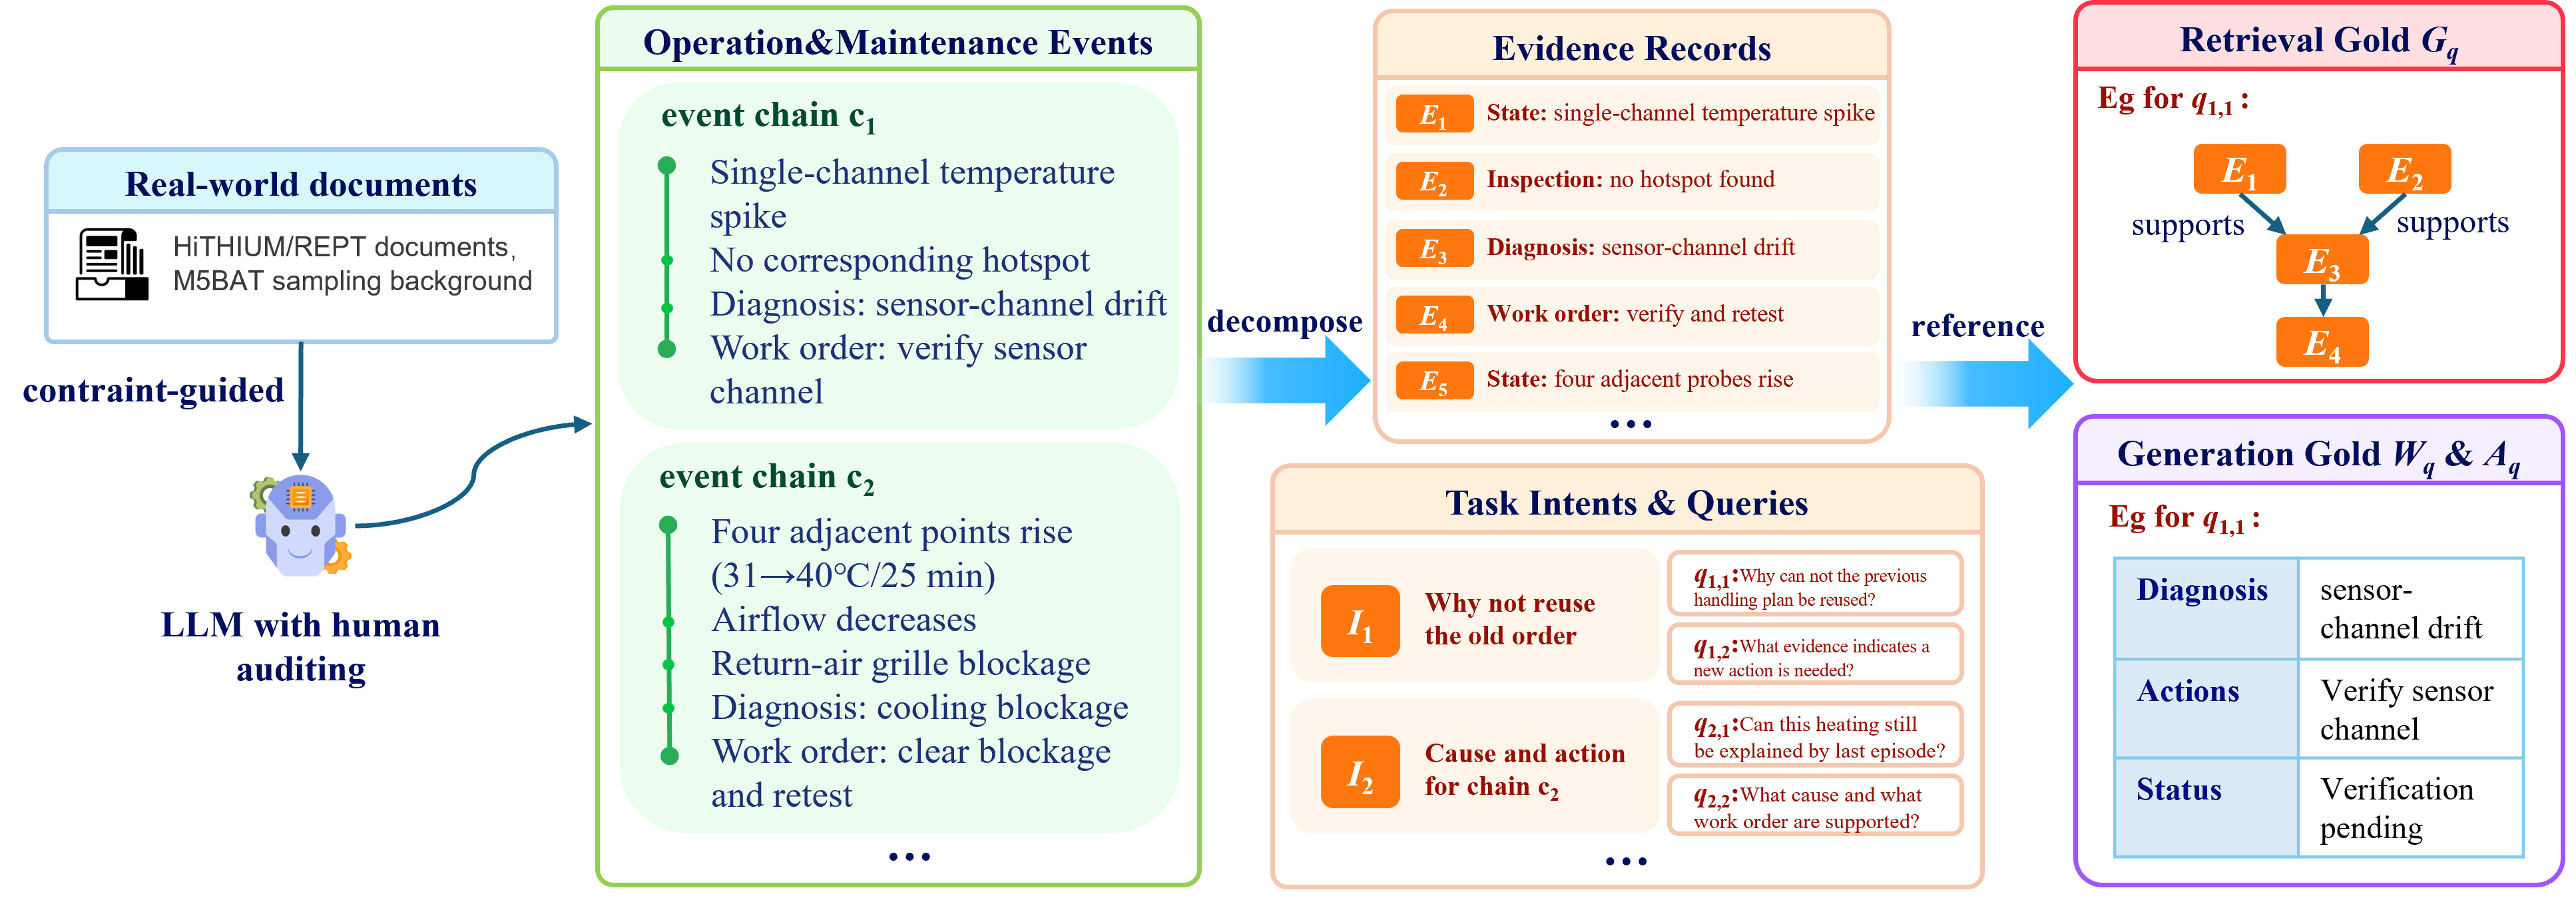
\includegraphics[width=0.98\textwidth]{figures/benchmark_design.png}
    % BEFORE: \caption{Construction pipeline and example for TEF-RAG v6 Semantic Benchmark v1. Public sources constrain the equipment and data background; an O\&M event chain $c$ is then constructed and used to derive evidence records $e_i$, task intents $I_j$, and queries $q_{j,p}$. Retrieval reference evidence flows and structured generation reference answers are subsequently created for each query to support retrieval and downstream generation evaluation.}
    \caption{Construction pipeline and example for the temporal O\&M benchmark. Public sources constrain the equipment and data background; an O\&M event chain $c$ is then constructed and used to derive evidence records $e_i$, task intents $I_j$, and queries $q_{j,p}$. Retrieval reference evidence flows and structured generation reference answers are subsequently created for each query to support retrieval and downstream generation evaluation.}
    \label{fig:benchmark_design}
\end{figure*}

\revhl{Table~\ref{tab:dataset_structure} lists the levels of the dataset. A chain contains the records of a complete O\&M process. Several task intents are defined on that chain, and two differently worded queries express each intent.}

\revhl{The reference annotations specify the information a query requires and the relations needed among its supporting records. Different records may satisfy the same requirement. Evaluation checks these requirements and relations across the retrieved set, so equivalent evidence can receive credit.}

\begin{table}[t]
\caption{Data hierarchy of the benchmark.}
\label{tab:dataset_structure}
\centering
\small
\begin{tabular}{@{}>{\centering\arraybackslash}p{0.24\columnwidth}>{\centering\arraybackslash}p{0.69\columnwidth}@{}}
\toprule
Level & Meaning \\
\midrule
Chain & A complete O\&M event process \\
Evidence & An atomic retrievable record with event time and availability time \\
Intent & A distinct O\&M information need defined on the same chain \\
Query & A differently worded query expressing the same intent \\
Reference flow & Key evidence requirements and their relation constraints \\
\bottomrule
\end{tabular}
\end{table}

\revhl{Across 100 target assets, the benchmark comprises 400 O\&M event chains with 3,888 retrievable records. These chains yield 1,200 task intents and 2,400 queries.} Development, validation, and test sets are split at the complete event-chain level. All queries derived from the same event chain appear in only one data split, preventing the same event content from appearing in both training and test data through different phrasings.

To evaluate retrieval under both ordinary and deliberately difficult temporal conditions, we divide the 400 event chains evenly into two difficulty strata. The standard subset contains relatively common combinations of temporal and O\&M conditions. The temporal-hard subset increases the frequency of cases involving late-arriving evidence, supersession, multi-episode ambiguity, cross-source complementary evidence, and persistent uncertainty.

\begin{table*}[t]
% BEFORE: \caption{Scale and split of TEF-RAG v6 Semantic Benchmark v1.}
\caption{Scale and split of the temporal O\&M benchmark.}
\label{tab:dataset_stats}
\centering
\small
\begin{tabular}{ccccc}
\toprule
Statistic & Development & Validation & Test & Total \\
\midrule
Authored chains & 240 & 80 & 80 & 400 \\
Primary intents & 720 & 240 & 240 & 1200 \\
Query rows & 1440 & 480 & 480 & 2400 \\
Evidence records & 2335 & 779 & 774 & 3888 \\
\bottomrule
\end{tabular}
\end{table*}

Public sources are used only to constrain cell type, typical operating ranges, and temporal sampling background, including energy-storage cell documents from HiTHIUM and REPT BATTERO and the RWTH M5BAT dataset~\cite{hithium2023v11,hithium2024v33,rept2025,rwth2026m5bat}. These sources are not used to define synthetic fault frequencies, station-level thresholds, or specific maintenance causal narratives in our benchmark.

\subsection{Structured Generation Evaluation}

\revhl{For generation evaluation, we prepare structured reference answers from the same O\&M event chains. Each answer is checked repeatedly against its chain and the required output format before it is finalized.}

\revhl{The two queries for an intent ask for the same diagnosis, action, and verification information, so both are evaluated against one reference answer. There are 720 reference answers for the 1,440 development queries, 240 for the 480 validation queries, and 240 for the 480 test queries.} Each output has two parts: a standardized work order and an action plan. The work order describes the diagnosis, recommended actions, applicable procedure, verification/uncertainty status, and evidence citations; the action plan consists of atomic actions and their dependencies.

\subsection{Baselines}
\label{sec:baselines}

To reduce confounding from differences outside the retrieval strategy, all methods first operate on the same evidence set that is eligible at the query time. We retain only records for the target asset satisfying
$t_e(e)\le t_q$ and $t_a(e)\le t_q$, and apply the same version-validity, withdrawal-status, and model-applicability constraints to procedure evidence. We compare six methods under this shared setup, with a final retrieval budget of at most five evidence records for every method.

\textbf{BM25.}
We use standard BM25 as the lexical retrieval baseline~\cite{robertson2009bm25}. For each query, a separate index is built over the eligible evidence set, with fixed parameters $k_1=1.5$ and $b=0.75$, and the five highest-scoring evidence records are returned directly.

\textbf{BGE Reranker.}
We first retrieve the Top-30 candidates using the same BM25 setup and then use \texttt{BAAI/bge-reranker-v2-m3} to rescore each $(\text{query},\text{evidence})$ text pair~\cite{chen2024bgem3,flagembedding2026reranker}. The top five records under the reranking score are selected. This baseline tests whether a general-purpose semantic reranker can compensate for the limitations of purely lexical retrieval.

\textbf{Fine-tuned BGE Reranker.}
To control for task-specific supervision, we additionally adapt the same BGE reranker using only development-split document-level relevance labels. Evidence records listed as acceptable for any required evidence group are treated as positives, while high-ranked eligible BM25 nonpositives are used as negatives; no relation or evidence-flow labels are used. We train rank-8 low-rank adapters on the attention query/value projections together with the classification head for two epochs, and select the checkpoint by validation normalized discounted cumulative gain at 5 (nDCG@5), with Recall@5 as a tie-breaker. At inference, this baseline uses the same BM25 Top-30 candidate pool and Top-5 output budget as the pretrained BGE reranker.

\textbf{Temporal-BM25.}
This baseline explicitly adds temporal matching to BM25 relevance. Its ranking score is
\begin{equation}
s_{\mathrm{TBM25}}(e,q)
=
\lambda\,\widetilde{s}_{\mathrm{BM25}}(e,q)
+
(1-\lambda)\,s_{\mathrm{time}}(e,q),
\end{equation}
where $\widetilde{s}_{\mathrm{BM25}}$ is the normalized BM25 score and $s_{\mathrm{time}}$ measures the match between the evidence event time and the target time implied by expressions such as years, time intervals, before/after, and current/latest in the query. For queries without explicit temporal intent, the temporal term is set to a constant, preserving the original BM25 ranking. Before final test evaluation, we compare $\lambda\in\{0.25,0.50,0.75\}$ on validation data, select $\lambda=0.25$, and fix this value for subsequent evaluation.

\textbf{TA-RAG.}
We adopt the Time-Aware RAG method of Lau et al.~\cite{lau2025tarag}. The method first decomposes a query into its topic and target time range, then restricts candidate documents using temporal-interval filtering and performs semantic retrieval and BGE reranking within the temporal candidate set. To adapt TA-RAG to our discrete O\&M events, each event time $t_e(e)$ is represented as a one-second half-open interval, and relative temporal expressions in a query are interpreted with $t_q$ as the reference time. In addition, the TA-RAG index is built only from evidence that satisfies the same temporal and procedure-applicability constraints as the other methods, preventing future records from affecting retrieval. 
Apart from substituting the language model used for temporal decomposition, the temporal decomposition, interval filtering, Nomic embedding, FAISS retrieval, and BGE reranking pipeline follows the public implementation.

\textbf{TEF-RAG.}
Our method applies learned evidence-pair screening, query-conditioned relation-graph construction, and nonlinear set-level ranking to the same eligible evidence set, and returns the candidate set with the highest overall evidence-flow score.

\subsection{Evaluation Metrics}
\label{sec:metrics}

\textbf{Retrieval.}
Recall@5 and nDCG@5 measure conventional retrieval relevance. Complete@5 measures whether the retrieved set contains all categories of key evidence required to complete the task. FlowComplete@5 further checks whether those records can form correct and mutually consistent evidence relations, thereby constituting a complete temporal evidence flow.

\textbf{Generation.}
We report four primary metrics in the main text: Field Macro F1 (strict), Action F1, Citation F1, and Evidence Support Recall. For the F1 measures, F1 denotes the harmonic mean of precision and recall. Field Macro F1 measures strict matching of key work-order fields, Action F1 measures normalized maintenance actions, and Citation F1 evaluates claim--evidence citation pairs. Evidence Support Recall measures the fraction of reference work-order and action claims requiring evidence support for which the generated output provides at least one acceptable supporting-evidence citation.

\subsection{Ablation Setup}

% BEFORE: To analyze the contribution of individual components, we conducted five ablations on 480 validation queries.
To analyze the contribution of individual components, we define five ablation variants and evaluate their frozen retrieval outputs on the same 480-query test split used for the main retrieval comparison. The ablations remove learned pair proposal, relation-graph-derived set features, hard-negative mining, the nonlinear set ranker, or both learned pair proposal and the nonlinear set ranker. The full model and all variants use the same Top-30 search pool, the same maximum number of evidence pairs sent to relation judging, the same relation-judging prompt and confidence threshold, and the same candidate-set construction procedure. The graph-feature ablation removes only relation-graph-derived set features and retrains the same RankNet; the hard-negative ablation keeps only the first training round; and the nonlinear-ranker ablation removes the learned set ranker and uses the preceding greedy evidence-set selector instead. The joint ablation removes both learned components: the pair proposer is replaced by the nonlearned pair prefilter, and the nonlinear ranker is replaced by the greedy evidence-set selector. Relation judging, relation-graph construction, and candidate-set construction remain unchanged. For the test evaluation, predictions are frozen before the test evaluator is accessed.
